\setcounter{chapter}{12}

\chapter{幂级数与Fourier级数}

幂级数和Fourier级数是两类典型的函数项级数,但不是全部。如果是一列函数
(以正整数为下标)依序累加起来,就可以称为函数项级数。

幂级数因为拥有良好的可计算性和局部收敛性,广泛用于各种未知函数的展开
和近似,是最基本和人类最熟悉的一类函数项级数。与幂级数相关的知识延续了
Taylor公式的有关理论。

Fourier级数是在现代工程中具有非常重要应用的函数项级数,特别是在信号处理
领域,离不开与其相关的许多工具,例如Fourier分析和Fourier变换
(Fourier Transformation,傅里叶变换)。

幂级数和Fourier级数在收敛特征上具有非常典型的差异,非常适合作为
后续学习和研究其他函数项级数的基础。

\section{幂级数及其应用}

\subsection{函数项级数的概念}

{\bf 数项级数(无穷级数):}一个{\it 数列}依序相加
$$S=\sum\limits_{n=1}^{\infty}u_n
=\lim\limits_{n\to\infty}\sum\limits_{k=1}^nu_k$$ 

{\bf 函数项级数:} 一个{\it 函数列}依序相加 
$$S(x)=\sum\limits_{n=1}^{\infty}u_n(x)
=\lim\limits_{n\to\infty}\sum\limits_{k=1}^nu_k(x)$$

{\bf 幂级数:} 一个{\it 整数次幂的幂函数列}依序相加
$$S(x)=\sum\limits_{n=0}^{\infty}a_n(x-x_0)^n$$ 

{\bf Fourier级数:} 一个{\it 三角函数列}依序相加
$$S(x)=\df{a_0}{2}+\sum\limits_{n=1}^{\infty}
(a_n\cos nx+b_n\sin nx)$$

\subsection{幂级数的概念与性质}

{\it 关于$x-x_0$的幂级数}(也称为{\it 以$x_0$为中心的幂级数}
\ps{幂级数也常被称为{\b Taylor级数},特别是如果$x_0$,也称为{\b Maclaurin级数}})记为,
$${\sum\limits_{n=0}^{\infty}a_n(x-x_0)^n}$$
其中:$a_n\in\mathbb{R}\,(n\in\mathbb{N})$,$x,x_0\in\mathbb{R}$。

以下的讨论中,不妨假设$x_0=0$,以
$${\sum\limits_{n=0}^{\infty}a_nx^n}$$
为代表研究幂级数的有关性质。

{\bf 例:}讨论如下幂级数的收敛区间:
\begin{enumerate}[(1)]
  \setlength{\itemindent}{1cm}
  \item $\sum\limits_{n=0}^{\infty}\df{x^n}{n!}$\hfill $(-\infty<x<+\infty)$
  \item $\sum\limits_{n=0}^{\infty}x^n$\hfill $(|x|<1)$
  \item $\sum\limits_{n=0}^{\infty}n!x^n$ \hfill $(x=0)$
\end{enumerate}

{\bf 注:}{\b 幂级数总是在某个(而不是多个)非空的区间上收敛,
且在忽略区间端点的情况下,该区间关于$x_0$对称。}

{\bf 定理13.1.1}(Abel定理)考虑幂级数
$$\sum\limits_{n=0}^{\infty}a_nx^n$$
\begin{enumerate}[(1)]
  \setlength{\itemindent}{1cm}
  \item 若在$x_0\ne 0$处该级数收敛,则对任意$|x|<|x_0|$,该级数绝对收敛; 
  \item 若在$x_0\ne 0$处该级数发散,则对任意$|x|>|x_0|$,该级数发散。 
\end{enumerate}

{\bf 推论:}存在收敛与发散的临界点:$x^*=\pm R$,使得幂级数在
以$x_0$为中心$R$为半径({\it 收敛半径})的对称区间内收敛,在其外发散。

{\bf 注:}在临界点处的收敛性需要单独判定!

{\bf 习题13.1-17:}设幂级数$\sumn a_nx^n$的收敛半径为$3$,求$\sumn na_n(x-1)^{n+1}$
的收敛区间。

{\bf 例:}设$a_n\geq0\;(n\in\mathbb{N})$,
若级数$\sum\limits_{n=0}^{\infty}a_n(x-x_0)^n$在$x_1$
处条件收敛,则其收敛半径$R=|x_1-x_0|$。

[提示]:该级数在$x_1$收敛,则可知其收敛半径至少为$|x_1-x_0|$。又其对应的绝对值
级数$\sum\limits_{n=0}^{\infty}a_n|(x_1-x_0)|^n$发散,由此可知,其收敛半径
不可能大于$|x_1-x_0|$。

{\bf 定理13.1.3-4:}若$\sum\limits_{n=0}^{\infty}a_nx^n$的系数满足
$$\limn\left|\df{a_{n+1}}{a_n}\right|=\rho
\quad\mbox{或}\quad\limn\sqrt[n]{|a_n|}=\rho,$$
则该幂级数的收敛半径$R=1/\rho$。

{\bf 例:}求下列幂级数的收敛区间
\begin{enumerate}[(1)]
  \setlength{\itemindent}{1cm}
  \item $\sum\limits_{n=0}^{\infty}\df{2+(-1)^n}{2^n}x^n$
  \item $\sum\limits_{n=0}^{\infty}\df{(x-1)^n}{2^nn}$
  \item $\sum\limits_{n=0}^{\infty}2^nx^{2n}$
  \item $\sum\limits_{n=0}^{\infty}x^{3n+1}$
\end{enumerate}

[提示]:(1)收敛半径$R=2$,区间端点对应的级数均发散,故收敛区间为$(-1,1)$;

(2)收敛半径$R=2$,$x=-1$时对应级数收敛,故收敛区间为$[-1,1)$;

(3)令$u=x^2$,易得$|u|<1$时级数收敛,从而$|x|<1$为收敛区间;

(4)原级数即为$x\sum\limits_{n=0}^{\infty}x^{3n}$,显然与
$\sum\limits_{n=0}^{\infty}x^{3n}$同敛散。令$u=x^3$,后一级数
即为$\sum\limits_{n=0}^{\infty}u^n$,收敛区间$|u|<1$。
最终可得原级数的收敛区间为$|x|<1$。

{\bf 注:}关于求幂级数的收敛域
\begin{enumerate}
  \setlength{\itemindent}{1cm}
  \item 一般步骤:{\b 先求收敛半径,再讨论区间端点的敛散性}
  \item 标准型幂级数: $\sum\limits_{n=0}^{\infty}a_nx^n$ 
  $${R=\limn\left|\df{a_n}{a_{n+1}}\right|}
  \quad\mbox{或}\quad {R=\df 1{\limn\sqrt[n]{|a_n|}}}$$ 
  \item 非标准型幂级数(缺项或通项为复合函数):先换元、整理,再求收敛半径 
  \item 比值极限不存在时,注意使用根值极限\ps{若
  $\limn\left|\df{a_{n+1}}{a_n}\right|$存在,
  $\limn\sqrt[n]{|a_n|}$必存在且与之相等}
\end{enumerate}

\subsection{幂级数的和函数}\ps{幂级数展开与求和都是各类考试的常见考点!}

{\bf 定理3:}(幂级数的运算性质)
\begin{enumerate}
  \setlength{\itemindent}{1cm}
  \item 两个幂级数的和在其收敛域的交集内收敛
  \ps{求和后的幂级数收敛域可能比原来的两个幂级数都大,例如:$\sumn x^n+\sumn(-1)x^n=0$}
  \item 幂级数逐项求导或求不定积分后收敛半径不变;\ps{收敛区间端点处的敛散性可能变化,要单独讨论!} 
  \item 幂函数的和函数在其收敛域上连续; 
  \item 幂函数逐项求导或求不定积分后,对应和函数分别为原和函数的导函数和原函数。
\end{enumerate}

{\bf 例:}已知
$$\df{1}{x+1}=\sum\limits_{n=0}^{\infty}(-x)^n\;(|x|<1),$$
求幂级数
$$\sum\limits_{n=1}^{\infty}\df{(-1)^{n-1}}{n}x^n$$
的和函数。由此证明:
$$\ln 2=1-\df 12+\df 13-\df 14+\ldots+\df{(-1)^n}{n}+\ldots$$

[解]:所给幂级数的收敛区间为$(-1,1]$。设其和函数为$S(x)$,则当$x\in(-1,1]$时,
\begin{align*}
	S'(x)&=\left[\sum\limits_{n=1}^{\infty}(-1)^{n-1}\df{x^n}{n}\right]'
	=\sum\limits_{n=1}^{\infty}\left[(-1)^{n-1}\df{x^n}{n}\right]'\\
	&=\sum\limits_{n=1}^{\infty}(-x)^{n-1}
	=\sum\limits_{n=0}^{\infty}(-x)^{n}=\df1{x+1},
\end{align*}
于是
$$S(x)=\dint_0^x\df1{t+1}\d t+S(0)=\ln|x+1|,$$
即为所求。当$x=1$时,
$$S(1)=\ln 2=1-\df 12+\df 13-\df 14+\ldots+\df{(-1)^n}{n}+\ldots.$$

{\bf 例:}求下列幂级数的和函数\ps{重点掌握,学会举一反三}
\begin{enumerate}[(1)]
  \setlength{\itemindent}{1cm}
  \item $\sum\limits_{n=0}^{\infty}\df{x^n}{n!}$
  \item $\sum\limits_{n=1}^{\infty}nx^n$
  \item $\sum\limits_{n=0}^{\infty}\df{x^n}{n+1}$
  \item $\sum\limits_{n=0}^{\infty}n^2x^n$
\end{enumerate}

[提示]:(1)收敛域$(-\infty,+\infty)$,
$$S'(x)=\left[\sum\limits_{n=0}^{\infty}\df{x^n}{n!}\right]'
=\sum\limits_{n=0}^{\infty}\left[\df{x^n}{n!}\right]'
=\sum\limits_{n=1}^{\infty}\df{x^{n-1}}{(n-1)!}=S(x),$$
又$S(0)=1$,求解微分方程初值问题,可得$S(x)=e^x$。

(2)收敛域$(-1,1)$,
$$
	\df{S(x)}x=\sum\limits_{n=1}^{\infty}nx^{n-1}
	=\sum\limits_{n=1}^{\infty}(x^{n})'
	=\left(\sum\limits_{n=1}^{\infty}x^{n}\right)'
	=\left(\df1{1-x}-1\right)'=\df1{(1-x)^2},
$$
从而
$$S(x)=\df{x}{(1-x)^2},\quad x\in(-1,1)$$

(3)收敛域$[-1,1)$,
$$
xS(x)=\sum\limits_{n=0}^{\infty}\df{x^n+1}{n+1}
=\sum\limits_{n=0}^{\infty}\dint_0^x t^n\d t
=\dint_0^x \sum\limits_{n=0}^{\infty}t^n\d t
=\dint_0^x \df1{1-t}\d t=-\ln|1-x|,
$$
故
$$S(x)=\left\{\begin{array}{ll}
	-\df{\ln|1-x|}x,&x\ne0\\
	1,&x=0.
\end{array}\right.$$

{\bf 例:}求数项级数$\sumn\sum\limits_{k=1}^n\df{k}{2^{n-1}}$的和。

[提示]:\ps{交换求和次序,可以使用初等方法求得级数的和}原级数即为
$$\sumn\df{n(n+1)}{2^n}.$$
考虑幂级数$\sumn n(n+1)x^n$,求出其和函数,然后令$x=\df12$即可。

\subsection{函数的幂级数展开}

函数$f(x)$在原点处的无穷阶Taylor展开式: 
$$f(x)=\sum\limits_{n=0}^{\infty}\df{f^{(n)}(0)}{n!}x^n$$
 称为:{\it $f(x)$在原点处的Taylor级数(Maclaurin级数)} 
 
{\bf 注:}展开的条件: $f(x)$在原点处无穷阶可导

{\bf 例:}求以下函数的Maclaurin级数\ps{重点掌握!}

\begin{enumerate}[(1)]
  \setlength{\itemindent}{1cm}
  \item $f(x)=1+x+4x^3-5x^{99}+x^{100}$ 
  \item $f(x)=(1-x)e^x$ 
  \item $f(x)=\sin(x-\pi/4)$ 
  \item $f(x)=\df 1{1-x^2}$ 
  \item $f(x)=\ln(2+x)$ 
  \item $f(x)=\arctan x$
\end{enumerate}

[提示]:(1)关于$x$的多项式函数的Maclaurin级数就是其自身。

注:若要求在$x=a$处的Taylor级数,则需要将$x$代换为$(x-a)+a$,然后将
原多项式展开为关于$x-a$的多项式即可。

(2)
$(1-x)e^x=\sum\limits_{n=0}^{\infty}(1-x)\df{x^n}{n!}
=1+\sum\limits_{n=1}^{\infty}\left[\df1{n!}-\df1{(n-1)!}\right]x^n
=1-\sum\limits_{n=1}^{\infty}\df1{n(n-2)!}x^n$
收敛域$(-\infty,+\infty)$.

(3)
$\sin(x-\pi/4)=\df{\sqrt2}2(\sin x-\cos x)
=\df{\sqrt2}2\sum\limits_{m=0}^{\infty}(-1)^m
\left(-\df{x^{2m}}{(2m)!}+\df{x^{2m+1}}{(2m+1)!}\right)$ 
收敛域$(-\infty,+\infty)$.

(4)记$u=x^2$
$$\df 1{1-x^2}=\df1{1-u}=\sum\limits_{n=0}^{\infty}u^n
\sum\limits_{n=0}^{\infty}x^{2n},$$
收敛域$(-1,1)$.

(5)记$u=\df x2$,则
$$\ln(2+x)=\ln2+\ln(1+u)
=\ln2+\sum\limits_{n=0}^{\infty}\df{(-1)^n}{n+1}u^{n+1}
=\ln2+\sum\limits_{n=0}^{\infty}\df{(-1)^n}{(n+1)2^n}x^{n+1},$$
收敛域$(-2,2]$

(6)由
$$\df1{1+x^2}=\sum\limits_{n=0}^{\infty}(-1)^nx^{2n},$$
两边同时积分,可得
$$\arctan x=\dint_0^x\left[\sum\limits_{n=0}^{\infty}(-1)^nt^{2n}\right]\d t
=\sum\limits_{n=0}^{\infty}(-1)^n\dint_0^xt^{2n}\d t
=\sum\limits_{n=0}^{\infty}\df{(-1)^n}{2n+1}x^{2n+1},$$
收敛域$(-1,1)$\ps{注意到$\arctan x$在$(-\infty,+\infty)$上处处无穷可导,但
其幂级数展开的收敛域只是$(-,1)$,这很好地说明了幂级数的局部收敛性}

{\bf 习题13.1-19:}将函数$f(x)=\arccos x$展开为$x$的幂级数,写出收敛区间,
并由此给出一个求圆周率$\pi$的公式。

[提示]:
$$(\arccos x)'=-(1-x^2)^{-\frac12}
=-\sum\limits_{n=0}^{\infty}
\left(\begin{array}{c} -\frac12 \\ n \end{array}\right)(-x^2)^n
=-\sum\limits_{n=0}^{\infty}\df{(2n-1)!!}{2n!!}x^{2n},
$$
收敛区间$(-1,1)$。
故
$$\arccos x-\arccos0
=-\dint_0^x\sum\limits_{n=0}^{\infty}\df{(2n-1)!!}{2n!!}t^{2n}\d t
=-\sum\limits_{n=0}^{\infty}\df{(2n-1)!!}{2n!!}\dint_0^xt^{2n}\d t
=-\sum\limits_{n=0}^{\infty}\df{(2n-1)!!}{2n!!(2n+1)}x^{2n+1},$$
收敛区间$[-1,1)$。

\subsection{幂级数的应用}

\subsubsection{【函数值的近似计算】}

\subsubsection{【积分的近似计算】}

\subsubsection{【解微分方程】}

{\bf 例:}求解初值问题:$$xy''+y'+xy=0,\;y(0)=1,\;y'(0)=0$$

\subsection{课堂练习}

{\bf 例:}判断正误
\begin{enumerate}[(1)]
  \setlength{\itemindent}{1cm}
  \item 幂级数在其收敛域上一定绝对收敛 \;{{$(\;\times\;)$}} 
  \item 设$\sum a_nx^n,\sum b_nx^n$的收敛半径分别为$R_1,R_2$,
  则$\sum(a_n+b_n)x^n$的收敛半径$R=\min\{R_1,R_2\}$ 
  \;{{$(\;\times\;)$}} 
  \item 幂级数与其逐项积分和逐项求导的幂级数的收敛域相同 
  \;{{$(\;\times\;)$}}
\end{enumerate}

[提示]:(1)幂级数在不包含收敛域端点的区间内绝对收敛;

(2)正确说法是$R\geq\min\{R_1,R_2\}$,例如:$a_n=-b_n$,则
$R=+\infty$;

(3)需要提出收敛域的端点!

{\bf 例:}若$\sum a_n(x-2)^n$在$x=-2$收敛,则在$x=5$处
\underline{\;{绝对收敛}\;};若在$x=-2$处条件收敛,
则收敛半径为\underline{\;{$4$}\;}

{\bf 例:}求函数项级数$\sum\limits_{n=1}^{\infty}
\sin\df 1 {3n}\left(\df{3+x}{3-2x}\right)^n$
的收敛域。

{\bf 例:}求级数$\sum\limits_{n=1}^{\infty}\df{n}{2^{n-1}}$的和。

{\bf 例:}将下列函数展开成Maclaurin级数,并求其收敛域
\begin{enumerate}[(1)]
  \setlength{\itemindent}{1cm}
  \item $f(x)=\arcsin x$
  \item $f(x)=\df 1{1+x+x^2}$
\end{enumerate}

[提示]:(2)$f(x)=\df{1-x}{1-x^3}$

\begin{shaded}
	{\bf 关于$\arctan x$的展开的讨论}
	
	1、先来看$\arctan x$的幂级数展开。由
	$$(\arctan x)'=\df1{1+x^2}
	=\sum\limits_{n=0}^{\infty}(-1)^nx^{2n}, \quad (|x|<1),$$
	两边积分
	$$\arctan x=\dint_0^x\sum\limits_{n=0}^{\infty}(-1)^nt^{2n}\d t
	+\arctan 0
	=\sum\limits_{n=0}^{\infty}(-1)^n\dint_0^xt^{2n}\d t+0
	=\sum\limits_{n=0}^{\infty}\df{(-1)^n}{2n+1}x^{2n+1},$$
	以上右侧的幂级数的收敛域为$[-1,1]$。故
	$${\b\arctan x=\sum\limits_{n=0}^{\infty}\df{(-1)^n}{2n+1}x^{2n+1},
	\quad |x|\leq1}$$
	
	\begin{center}
		\resizebox{!}{5cm}{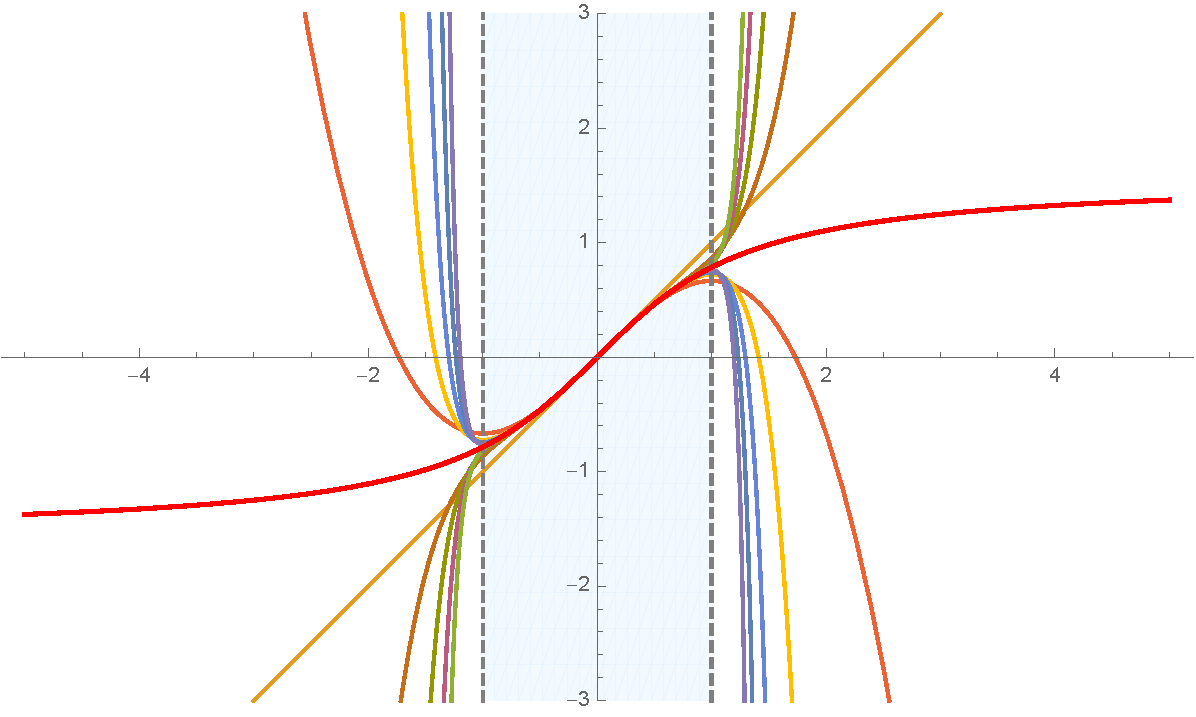
\includegraphics{./images/ch13/arctan-1.pdf}}
	\end{center}
	
	2、下面换一种方式
	$$(\arctan x)'=\df1{1+x^2}=\df1{x^2}\df1{1+\frac1{x^2}}
	=\df1{x^2}\sum\limits_{n=0}^{\infty}\df{(-1)^n}{x^{2n}}
	=\sum\limits_{n=0}^{\infty}\df{(-1)^n}{x^{2n+2}}, \quad (|x|>1),$$
	当$x>1$时,两边积分
	\begin{align*}
	\arctan x&=\arctan(+\infty)-
	\dint_x^{+\infty}\sum\limits_{n=0}^{\infty}\df{(-1)^n}{t^{2n+2}}\d t\\
	&=\df{\pi}2-\sum\limits_{n=0}^{\infty}{(-1)^n}\dint_x^{+\infty}\df{\d
	t}{t^{2n+2}} =\df{\pi}2-\sum\limits_{n=0}^{\infty}\df{(-1)^{n}}{(2n+1)x^{2n+1}},
	\end{align*}
	以上右侧级数的收敛域为$x\geq 1$;同理,$x<1$时,
	$$\arctan x=-\df{\pi}2
	-\sum\limits_{n=0}^{\infty}\df{(-1)^{n}}{(2n+1)x^{2n+1}},$$
	右侧级数的收敛域为$x\leq -1$。综上
	$${\b\arctan x=\mathrm{sgn}(x)\df{\pi}2-\sum\limits_{n=0}^{\infty}
	\df{(-1)^{n}}{(2n+1)x^{2n+1}},\quad |x|\geq1.}$$
	
	\begin{center}
		\resizebox{!}{5cm}{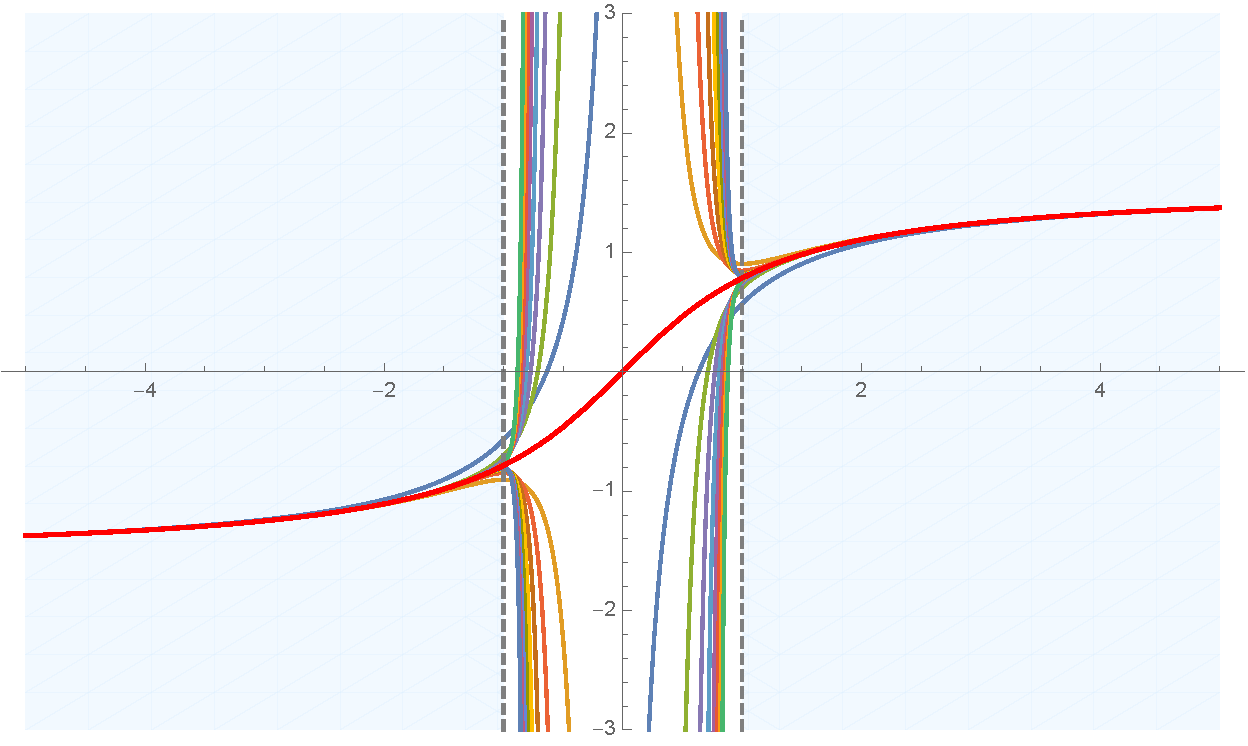
\includegraphics{./images/ch13/arctan-2.pdf}}
	\end{center}
	
	3、至此我们可以看到,同一个函数$\arctan x$可以由两种不同的展开式,似乎
	与函数的幂级数展开式的唯一性矛盾,真的是这样吗?
	
	答案是否定的!因为我们得到的第二个展开式并不是幂级数。
	
	对于$\arctan x$来说,其幂级数展开的“有效”区间(收敛域)只是$[-1,1]$,而
	$\arctan x$在定义区间$(-\infty,+\infty)$内是无穷次可导的,用幂级数展开
	只能表示$\arctan x$的一部分。这个现象说明,
	{\it 幂级数展开的局部性可以有两种理解,一是越靠近展开的位置结果越精确,
	二是这种展开很可能不是对函数的定义域全局有效的}。
	
	对$\arctan x$来说,以上两个展开式恰好构成了其定义域上完整的表示,使
	我们计算其在任一点处的函数值成为了可能。
% 	也即
% 	$$\arctan x=\left\{\begin{array}{ll}
% 		\sum\limits_{n=0}^{\infty}\df{(-1)^n}{2n+1}x^{2n+1},& |x|\leq 1;\\
% 		\mathrm{sgn}(x)\df{\pi}2-\sum\limits_{n=0}^{\infty}
% 		\df{(-1)^{n}}{(2n+1)x^{2n+1}},&
% 		|x|\geq 1.
% 	\end{array}\right.$$
\end{shaded}

\section{Fourier级数}

\subsection{三角级数与Fourier级数}

幂级数:{\it 对无穷次可导函数的局部逼近}

$${f(x)=\sum\limits_{n=0}^{\infty}\df{f^{(n)}(x_0)}{n!}(x-x_0)^n}$$
\begin{center}
	\resizebox{!}{5cm}{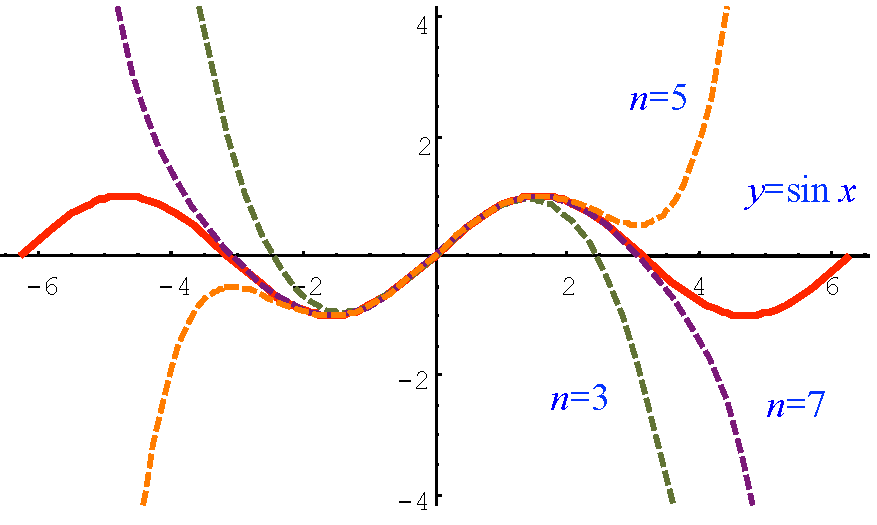
\includegraphics{./images/ch13/sinm.pdf}}
\end{center}

Fourier级数:{\it 对周期函数的整体逼近}

% {\bf Insight:}利用周期运动来逼近周期运动会有更好的整体逼近效果!

{\it 简谐振动:} 例如弹簧振子、钟摆
$$f(t)=A\sin(\omega t+\varphi)$$
其中:$A$为振幅;$\omega$为角频率;$\varphi$为初相位。
记$x=\omega t,\,a=A\sin\varphi,\,b=A\cos\varphi$, 则
$${g(x)=f(t)=a\cos x+b\sin x}$$

{\it Daniel Bernoulli (1700-1782):}任何复杂的振动都可以分解成一系列简谐振动之和

{\it Joseph Fourier (1768-1830):}“任意”函数都可以展开成三角级数

$${f(t)=A_0+\sumn A_n\sin(n\omega t+\varphi_n)}$$

{\bf 三角级数与周期函数的整体逼近}

$${f(x)=\df{\pi}{4}\mathrm{sgn}(x),\;(x\in[-\pi,\pi])
\;{\sim\;\sum\limits_{k=1}^n\df{\sin(2k-1)x}{2k-1}}}$$

\begin{center}
	\resizebox{!}{4cm}{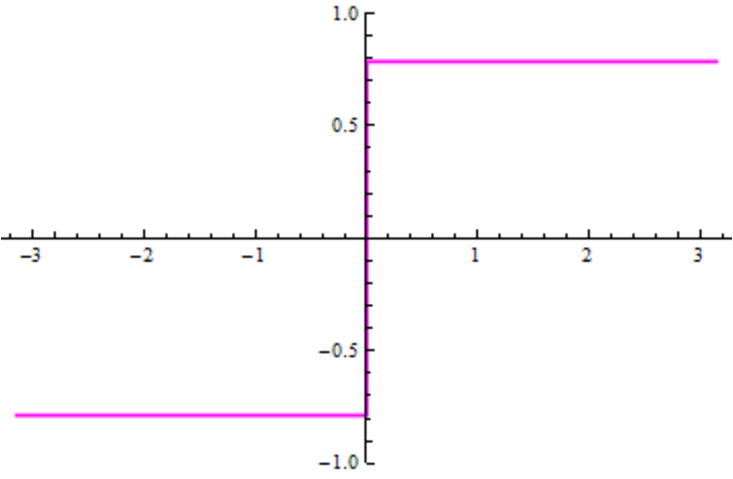
\includegraphics{./images/ch13/fsgn/f0.pdf}}
	\quad
	\resizebox{!}{4cm}{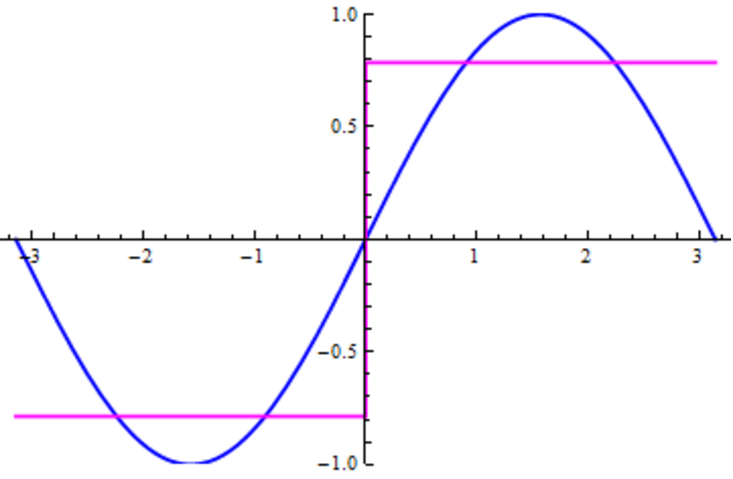
\includegraphics{./images/ch13/fsgn/f1.pdf}}
	
	\resizebox{!}{4cm}{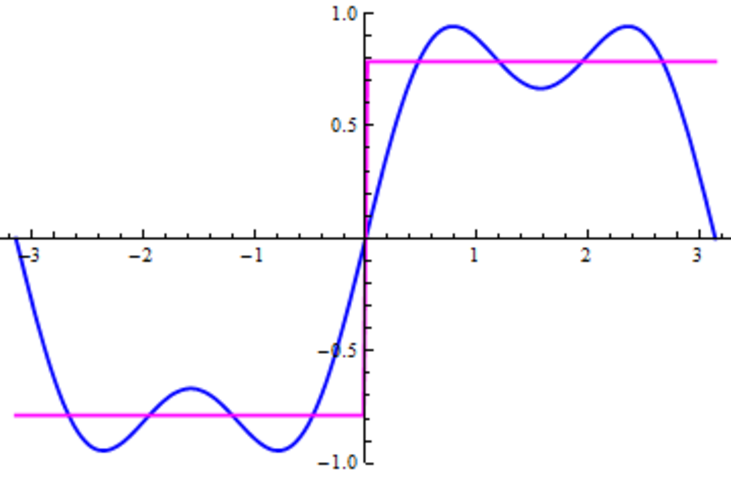
\includegraphics{./images/ch13/fsgn/f2.pdf}}
	\quad
	\resizebox{!}{4cm}{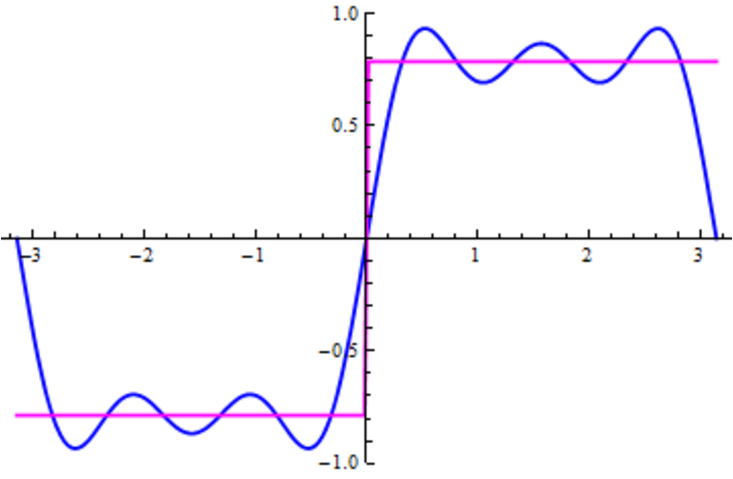
\includegraphics{./images/ch13/fsgn/f3.pdf}}
	
	\resizebox{!}{4cm}{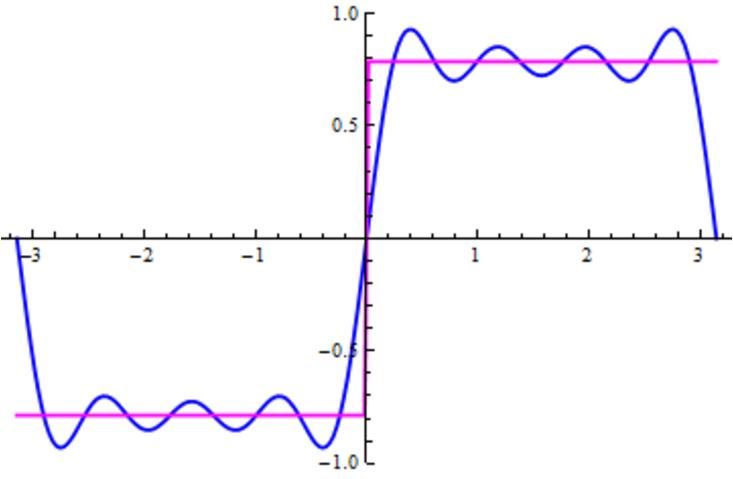
\includegraphics{./images/ch13/fsgn/f4.pdf}}
	\quad
	\resizebox{!}{4cm}{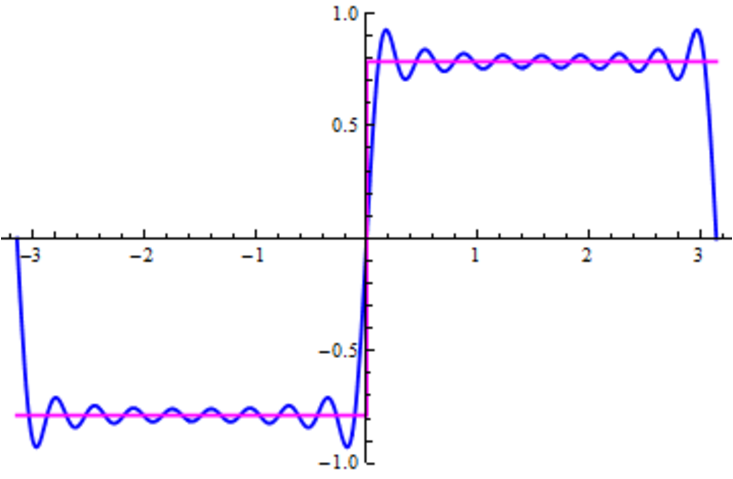
\includegraphics{./images/ch13/fsgn/f5.pdf}}
\end{center}

\begin{shaded}
	{\bf Fourier's Motivation}
	
	以下内容引自Wikipedia关于Fourier Series的条目。
	
	{\it
		The Fourier series is named in honour of \underline{Jean-Baptiste Joseph 
		Fourier} (1768–1830), who made important contributions to the 
		study of \underline{trigonometric series}(三角级数), after preliminary
		investigations by \underline{Leonhard Euler}, 
		\underline{Jean le Rond d'Alembert}, and \underline{Daniel Bernoulli}.
		{\b Fourier introduced the series for the purpose of solving the 
		\underline{heat equation}(热方程) in a metal plate}, publishing his initial
		results in his 1807 Mémoire sur la propagation de la chaleur dans 
		les corps solides (Treatise on the propagation of heat in 
		solid bodies,《热的解析理论》), and publishing his Théorie analytique de 
		la chaleur (Analytical theory of heat) in 1822. The Mémoire 
		introduced Fourier analysis, specifically Fourier series. 
		Through Fourier's research the fact was established that 
		an arbitrary (continuous) function can be represented by 
		a trigonometric series(任意给定的函数均可以表示为一个三角级数). 
		The first announcement of this 
		great discovery was made by Fourier in 1807, before the 
		French Academy. Early ideas of decomposing a periodic 
		function into the sum of simple oscillating functions date 
		back to the 3rd century BC, when ancient astronomers proposed 
		an empiric model of planetary motions, based on deferents and 
		epicycles.

		The heat equation is a partial differential equation(偏微分方程). 
		Prior to Fourier's work, no solution to the heat equation 
		was known in the general case, although particular solutions 
		were known if the heat source behaved in a simple way, in 
		particular, if the heat source was a sine or cosine wave. 
		These simple solutions are now sometimes called eigensolutions. 
		Fourier's idea was to model a complicated heat source as a 
		superposition (or linear combination) of simple sine and 
		cosine waves, and to write the solution as a superposition 
		of the corresponding eigensolutions. This superposition or 
		linear combination is called the Fourier series.
		
		From a modern point of view, Fourier's results are somewhat 
		informal, due to the lack of a precise notion of function and 
		integral in the early nineteenth century. Later, \underline{Peter 
		Gustav Lejeune Dirichlet} and \underline{Bernhard Riemann} expressed Fourier's 
		results with greater precision and formality.
		
		Although the original motivation was to solve the heat equation, 
		it later became obvious that the same techniques could be applied 
		to a wide array of mathematical and physical problems, and 
		especially those involving linear differential equations with 
		constant coefficients, for which the eigensolutions are sinusoids. 
		The Fourier series has many such applications in electrical 
		engineering(电子工程), vibration analysis(振动分析), acoustics(声学), 
		optics(光学), signal processing(信号处理), image processing(图像处理), 
		quantum mechanics(量子力学), econometrics(计量经济学), 
		thin-walled shell theory(?), etc.
	}
	
	下面据说是Fourier最初的工作:
	
	考虑位于平面区域$[0,\pi]\times[0,\pi]$上的金属薄片,已知其上的温度分布$T(x,y)$满足热方程
	$$\df{\p^2T}{\p x^2}+\df{\p^2T}{\p y^2}=0,$$
	以及如下的边界条件:
	$$T(x,0)=T(0,y)=T(\pi,y)=0,\quad T(x,\pi)=x,$$
	求$T(x,y)$。
	
	\begin{center}
% 		\resizebox{!}{5cm}{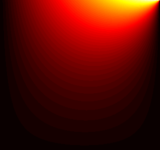
\includegraphics{./images/ch13/Fourier_heat_in_a_plate.pdf}}
% 		\quad
		\resizebox{!}{6cm}{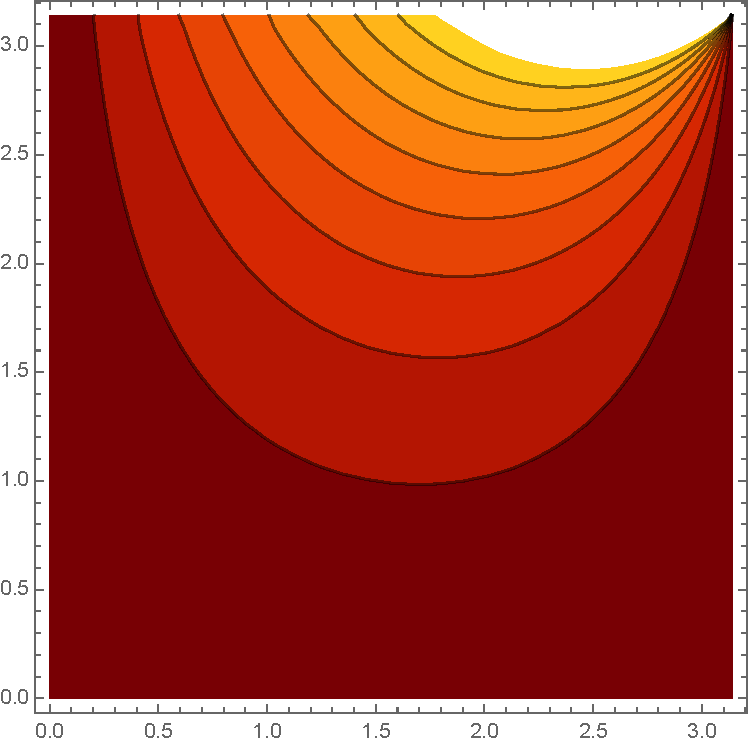
\includegraphics{./images/ch13/solarPlate.pdf}}
		
		{\it $T(x,y)$的等温线——从红到白,温度逐渐升高}
	\end{center}
	
	注:$T(x,y)$可以理解为处于热平衡状态(金属片上不再发生热传导)时的温度分布。
	这里所考虑的方程只是热方程的一种简单形式,但以下的方法为求解更为
	复杂和一般的问题提供了思路。
	
	Fourier的思路是这样的:很久以来,人们都知道如果以上的最后一个边界条件改为
	$$T(x,\pi)=\sin nx,\;n=1,2,3,\ldots,$$
	其他条件均不变,则热方程存在如下的解(一般称为{\it 本征解})
	$$T(x,y)=\sin nx\df{\sinh ny}{\sinh n\pi}
	=\sin nx\cdot\df{e^{ny}-e^{-ny}}{e^{n\pi}-e^{-n\pi}}.$$
	
	Fourier注意到这样一个事实,给定不同的边界条件,其叠加后产生的温度分布也是可以叠加的。以
	我们这里所考虑的问题为例,也即:给定四个边上的多组边界函数$(a_i(x),b_i(x),c_i(x),
	d_i(x)),(i=1,2,\ldots,n)$,若其对应的温度分布分别为$T_i(x,y),(i=1,2,\ldots,n)$,
	则对于叠加后边界函数$\sum\limits_{i=1}^n(a_i(x),b_i(x),c_i(x),d_i(x))$,其相应的
	温度分布就是所有对应温度分布的叠加,也即:$\sum\limits_{i=1}^nT_i(x,y)$。
	
	因此,Fourier想到,如果$x$可以表示为$\{\sin nx|n=1,2,3,\ldots\}$的叠加
	(线性组合)形式,那么利用同样的线性组合,由这些边界函数对应的本征解就可以叠加构造
	出$x$对应的问题的解。
	
	最终,Fourier利用如下的三角级数(如何得到类似这样的三角级数,正是我们需要在高等数学课程
	中学习的)
	$$x=2\sumn\df{(-1)^{n+1}}{n}\sin{nx},\quad x\in[0,\pi],$$
	得到了最终的温度分布
	$$T(x,y)=2\sumn\df{(-1)^{n+1}}{n}\sin{nx}
	\cdot\df{e^{ny}-e^{-ny}}{e^{n\pi}-e^{-n\pi}}.$$
\end{shaded}

{\bf 三角级数}
$${\df{a_0}{2}+\sumn(a_n\cos nx+b_n\sin nx)}$$ 

{\bf 定理:}
三角函数序列$A=\{\cos kx,\sin kx|k=1,2,\ldots\}$具有{\it 正交性} ,
即:任意$f(x),g(x)\in A$,
$$\dint_{-\pi}^{\pi}f(x)g(x)dx=\left\{\begin{array}{ll}
0,\;& f(x)\ne g(x)\\ \pi\;& f(x)=g(x)
\end{array}\right.$$

{\bf 注:}将常值函数$1$加入$A$中,不改变其正交性,只是$1$不满足
平方积分等于$\pi$(而是等于$2\pi$)。因此,在Fourier展开式中,与$1$对应的系数$a_0$
需要除以$2$。

{\bf 定理:}若函数$f(x)$可展成如下三角级数
$$\df{a_0}{2}+\sumn(a_n\cos nx+b_n\sin nx),$$
且该三角级数可逐项积分, 则
$${\b\left\{\begin{array}{ll}
a_n=\df1{\pi}\dint_{-\pi}^{\pi}f(x)\cos nx\d x,\;& n=0,1,2,\ldots\\[5pt]
b_n=\df1{\pi}\dint_{-\pi}^{\pi}f(x)\sin nx\d x,\;& n=1,2,\ldots
\end{array}\right.}$$

\begin{shaded}
	{\bf 利用正交函数列构造函数项级数}
	
	如果能够找到与$A$类似的一个正交函数序列,则可以利用以上定理的
	思想来构造类似Fourier级数的函数项级数。
	
	例如:$B=\{\xi_n(x)\}$,其中
	$\xi_n(x),\;n=0,1,2,\ldots$均为以$2$为周期的函数,且在$x\in[0,2]$上,
	$$
		\left\{\begin{array}{rl}
			\xi_0(x)&=1\\
			\xi_1(x)&=(-1)^{[x]}\\
			\xi_2(x)&=(-1)^{[2x]}\\
			\xi_3(x)&=(-1)^{[4x]}\\
			\ldots&\ldots\\
			\xi_n(x)&=(-1)^{[2^nx]}\\
			\ldots&\ldots
		\end{array}\right.
	$$
	其中$[x]$表示下取整函数,也即不大于$x$的最大的整数。
	
	可以证明任意$f,g\in B$,均满足:
	$$\dint_0^{2}f(x)g(x)\d x=
	\left\{\begin{array}{ll}
		0,& f\ne g\\ 2,& f=g
	\end{array}\right.$$
	
	参考Fourier级数的有关定理,给以类似地给出如下结论:
	{\bf 定理:}对任意以$2$为周期的函数$f(x)$,若其可以表示为
	$$f(x)\sim\sum\limits_{n=0}^{\infty}u_n\xi_n(x),$$
	且右端级数可以逐项积分,则
	$$
	u_n=\df12\dint_0^2f(x)\xi_n(x)\d x,\;n=0,1,2,\ldots.
	$$
\end{shaded}

{\bf 例:}已知$f(x)=\left\{\begin{array}{ll}
	x,& x\in[-\pi,\pi),\\ f(x+2\pi)& \mbox{其他}
\end{array}\right.$,求其对应的Fourier级数。

[解]:对$n=0,1,2,\ldots$,
$$a_n=\df1{\pi}\dint_{-\pi}^{\pi}x\cos nx\d x=0.$$
对$n=1,2,\ldots$,
\begin{align*}
	b_n&=\df1{\pi}\dint_{-\pi}^{\pi}x\sin nx\d x
	=-\df1{n\pi}\dint_{-\pi}^{\pi}x\d\cos nx\\
	&=-\df1{n\pi}\left[x\cos nx|_{-\pi}^{\pi}
	-\dint_{-\pi}^{\pi}\cos nx\d x\right]=2\df{(-1)^{n+1}}n
\end{align*}
综上,所求Fourier级数为
$$2\sumn\df{(-1)^{n+1}}n\sin nx.$$

{\bf 例:}$f(x)$以$2\pi$为周期,且在$[-\pi,\pi)$内$f(x)=\df{\pi}{4}\mathrm{sgn}(x)$,
求其Fourier级数。

{\bf 注:}
\begin{enumerate}[(1)]
  \setlength{\itemindent}{1cm}
  \item {\b $[-\pi,\pi]$上的奇函数的Fourier级数只含有正弦项, 称为{\it 正弦级数}}
  \item {\b $[-\pi,\pi]$上的偶函数的Fourier级数只含有余弦项, 称为{\it 余弦级数}}
  \item 计算以$2\pi$为周期的函数的Fourier级数,积分区间选择任意一个长度为$2\pi$
  的连续区间即可,也即:任取常数$x_0\in\mathbb{R}$,均有
  	$${\b\left\{\begin{array}{ll}
		a_n=\df1{\pi}\dint_{x_0}^{x_0+2\pi}f(x)\cos nx\d x,\;& n=0,1,2,\ldots\\[5pt]
		b_n=\df1{\pi}\dint_{x_0}^{x_0+2\pi}f(x)\sin nx\d x,\;& n=1,2,\ldots
  	\end{array}\right.}$$
  \item {\b 只在有限点处取值不同的函数,Fourier级数相同},因为改变函数在有限点
  处的值,其定积分不变。
  \item Fourier展开具有{\it 线性性},也即:$f(x)+g(x)$的Fourier系数等于$f(x)$和
  $g(x)$的Fourier系数的和
\end{enumerate}

{\bf 例:}已知$f(x)=\left\{\begin{array}{ll}
	e^x,& x\in[0,2\pi),\\ f(x+2\pi)& \mbox{其他}
\end{array}\right.$,求其对应的Fourier级数。

[提示]:根据$f(x)$的特征,应考虑使用以上注(3)中的公式,也即
$$a_n=\df1{\pi}\dint_{0}^{2\pi}e^x\cos nx\d x,\; n=0,1,2,\ldots,$$
$$b_n=\df1{\pi}\dint_{0}^{2\pi}e^x\sin nx\d x,\; n=1,2,\ldots.$$
如果使用常见的公式形式,则应该为
$$a_n=\df1{\pi}\left[\dint_{-\pi}^{0}e^{x+2\pi}\cos nx\d x+
\dint_{0}^{\pi}e^x\cos nx\d x\right],\; n=0,1,2,\ldots,$$
$$b_n=\df1{\pi}\left[\dint_{-\pi}^{0}e^{x+2\pi}\sin nx\d x+
\dint_{0}^{\pi}e^x\sin nx\d x\right],\; n=1,2,\ldots.$$

{\bf 例:}将下列函数展成Fourier级数
\begin{enumerate}[(1)]
  \setlength{\itemindent}{1cm}
  \item $f(x)=1+3\sin x+4\cos 3x-9\sin 2x$
  \item $f(x)=\sin^4x$
\end{enumerate}

[提示]:(2)利用半角/倍角公式降低幂次
\begin{align*}
	\sin^4x&=\left(\df{1-\cos2x}2\right)^2
	=\df14\left(1-2\cos2x+\cos^22x\right)\\
	&=\df14\left(1-2\cos2x+\df{1+\cos4x}{2}\right)\\
	&=\df38-\df12\cos2x+\df18\cos4x
\end{align*}
即为所求。

{\bf 注:}{\b 以$2\pi$为周期的一次三角多项式的Fourier级数是其自身}

\subsection{Fourier级数的收敛性}

{\bf 定理13.2.1}(Dirichlet收敛条件)$f(x)$以$2\pi$为周期, 在$[-\pi,\pi]$上其
{\it 分段连续}且{\it 仅有有限多个极值点}\ps{$\sin\df1x$在原点的的任意邻域内均有
无穷多个极值点,不满足该条件!}, 
则$f(x)$的Fourier级数处处收敛,
 其和函数
$$S(x) =\df{f(x+0)+f(x-0)}{2}.$$

{\bf 注:}根据定理条件,可知$f(x)$不可能有第二类间断点,故以上结论可以表述为:
$S(x)$在$f(x)$的连续点处收敛于$f(x)$,在$f(x)$的不连续点处收敛于其左右极限的中点。

{\bf 例:}试写出函数
$$f(x)=\left\{\begin{array}{rl}
	-\df{\pi}{4},\; & -\pi\leq x<0\\[8pt]
	\df{\pi}{4},\; & 0\leq x<\pi
\end{array}\right.$$
的Fourier级数的和函数。

[解]:
$${S(x)=\left\{\begin{array}{ll}
	-\pi/4,\;& -\pi<x<0\\
	\pi/4,\;& 0<x<\pi\\
	0,\; & x=0,\pm\pi
\end{array}\right.}$$

{\bf 例:}设周期函数$f(x)$在一个周期内的表达式为
$$f(x)=\left\{\begin{array}{ll}
	-1,\;& -\pi<x\leq 0\\
	1+x^2,\; & 0<x\leq\pi
\end{array}\right.$$
写出该函数在$[-\pi,\pi]$上的和函数$S(x)$,并求
$S(5\pi/2),S(7\pi/2),S(7\pi)$和$S(2008\pi)$的值。

{\bf 利用Fourier级数求特殊级数的和}

{\bf 例:}由
$$\df{\pi}4=\sum\limits_{m=1}^{\infty}
\df{\sin(2m-1)x}{2m-1},\;0<x<\pi,$$
 令$x=\pi/2$, 可得
$$\df{\pi}4=1-\df 13+\df 15-\df 17+\ldots
+(-1)^{m-1}\df 1{2m-1}+\ldots$$

{\bf 例:}设$f(x)=|x|\;(-\pi\leq x\leq \pi)$的Fourier级数,并由此
证明:
$$\df{\pi^2}{6}=1+\df 1{2^2}+\df 1{3^2}+\ldots+\df 1{n^2}+\ldots$$
$${|x|=\df{\pi}2-\df 4{\pi}\sum\limits_{m=1}^{\infty} 
\df{\cos(2m-1)x}{(2m-1)^2},\;-\pi\leq x\leq \pi}$$

{\bf 例:}设周期函数$f(x)$在一个周期内的表达式为
$$f(x)=e^x\;(x\in[0,2\pi]),$$
试将其展成Fourier级数,并求下列数值级数的和:
$$\sum\limits_{n=1}^{\infty}\df1{1+n^2}$$

Fourier展开给出了求函数的三角级数的方法,但是它需要满足一个基本的条件:
$f(x)$以$2\pi$为周期。

在现实问题中,很多函数并不是周期函数,即使是周期函数,也未必一定以$2\pi$
为周期。针对这样的函数,可以通过对函数(定义区间)的延拓或放缩,使之满足Fourier
展开的条件,然后间接地求得其对应的三角级数。

\subsection{函数的延拓及其Fourier展开}

{\bf 1、周期延拓}

若$f(x)$为定义在$(-\pi,\pi)$上的函数,满足Dirichlet条件。严格来说,为了
对其进行Fourier展开,需要将其视为某个周期函数$F(x)$的一部分,$F(x)$在
$(-\pi,\pi)$上定义与$f(x)$完全相同。这样一来,$F(x)$对应的Fourier级数
也就是$f(x)$的三角级数展开。

{\bf 2、奇(偶)延拓}

考虑定义在$(0,\pi)$上的函数$f(x)$,且在其上满足Dirichlet条件。为了对其进行
Fourier展开,只需为其补充$[-\pi,0]$上的定义,再利用周期延拓构造一个
以$2\pi$在为周期的函数$F(x)$。最后,将$F(x)$作Fourier展开,
其中$(0,\pi)$上的部分即为$f(x)$的三角级数展开。

在补充$[-\pi,0]$上的函数定义时,我们有许多的选择,理论上讲,任意在$[-\pi,0]$
满足Dirichlet条件的函数都是可能的选择。

在前面关于Fourier级数的讨论中我们曾提到,若给定的函数为奇(偶)函数,则
其Fourier级数中只含正(余)弦项,对应的级数可以称为正(余)弦级数。在接下来
的讨论中,我们将着重讨论一下展开后的三角级数分别为正弦和余弦级数的情形,
对应的延拓方式分别称为奇延拓和偶延拓。

具体来说,{\b 设$f(x)$在$(0,\pi)$上满足Dirichlet条件,令
$$F(x)=\left\{\begin{array}{ll}
  	f(x),\;& x\in(0,\pi)\\
  	0,\;& x=0,-\pi\\
  	\pm f(-x),\;& x\in(-\pi,0)
  \end{array}\right.$$
且
  $$F(x+2\pi)=F(x)\;(-\infty<x<\infty).$$
这样一来,$F(x)$就是满足Dirichlet条件的偶(奇)周期函数,其Fourier级数为
余(正)弦级数,其中在$(0,\pi)$内的部分即为$f(x)$对应的余(正)弦级数。}

{\bf 例:}设函数$f(x)=x+1\,(x\in(0,\pi))$,试将其分别展开为正弦和余弦级数。

\begin{center}
	\resizebox{!}{2.7cm}{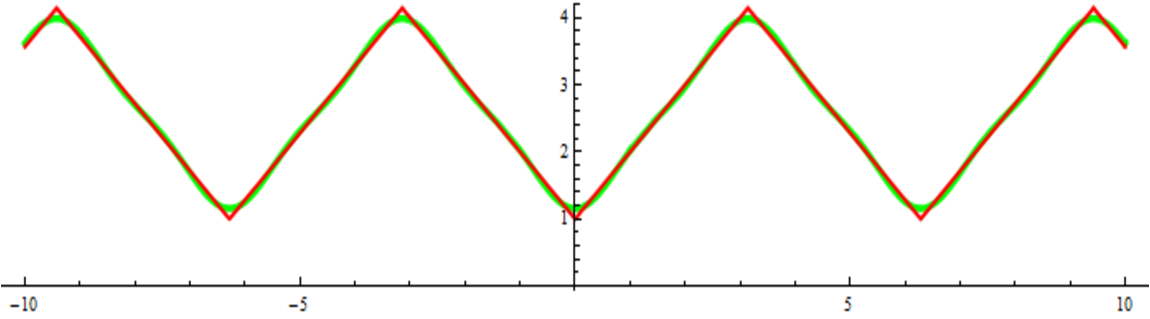
\includegraphics{./images/ch13/cs.pdf}} 
	
	\resizebox{!}{2.7cm}{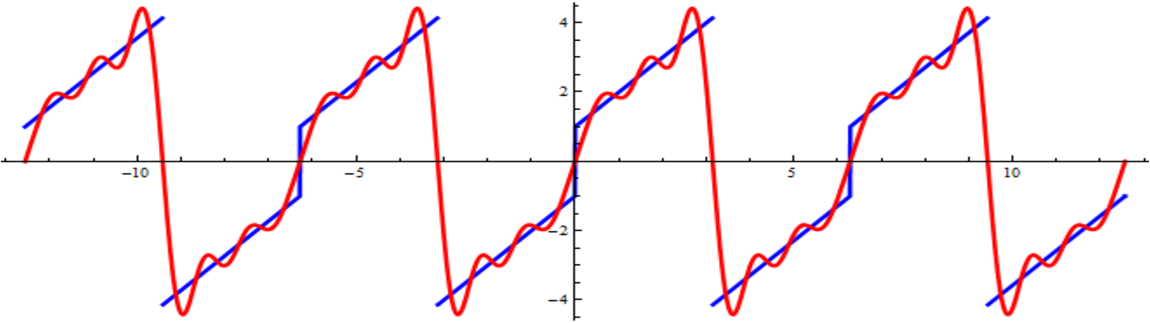
\includegraphics{./images/ch13/ss.pdf}}
\end{center}

{\bf 注:}{\b 对于同一个定义在$(0,\pi)$上的函数,采用不同的延拓方式展开成
三角级数,所得的结果可能是不同的!这和Fourier展开的唯一性并不矛盾,因为
对于延拓后生成的函数来说,其对应的Fourier级数是唯一的。}

{\bf 例:}设$f(x)=\pi x-x^2\,(0<x<\pi)$,又设$S(x)$是$f(x)$在$(0,\pi)$内以
$2\pi$为周期的正弦级数展开式的和函数,求当$x\in(\pi,2\pi)$时$S(x)$的表达式。

\subsection{周期为$2l$的Fourier级数}

接下来考虑任意周期为$2l$的函数$f(x)$的三角级数展开问题,其中$l\ne0$且不一定等于$\pi$。

从数学的角度,只需通过一些坐标的伸缩即可达到展开的目的。具体来说,令$t=\df{\pi}{l}x$,
则$g(t)=f\left(\df{l}{\pi}t\right)$ 是以$2\pi$为周期的函数。 
对$g(t)$做Fourier展开,由其展开式可变换得到$f(x)$的展开式。

$$f(x)=\df{a_0}2+\sumn\left(a_n\cos\df{n\pi}lx+b_n\sin\df{n\pi}lx\right)$$
其中
$$\left\{\begin{array}{ll}
a_n=\df1{l}\dint_{-l}^{l}f\left(\df{\pi}lx\right)
\cos n\left(\df{\pi}lx\right)\d x,\;&
n=0,1,2,\ldots\\[5pt] b_n=\df1{l}\dint_{-l}^{l}f\left(\df{\pi}lx\right)
\sin n\left(\df{\pi}lx\right)\d x,\;& n=1,2,\ldots
\end{array}\right.$$

需要注意的是,此时得到的$f(x)$的展开式,其基函数并不是以$2\pi$为周期的三角函数,
而是以$2l$为周期的三角函数。

{\bf 例:}将函数$f(x)=x\,(0<x<1)$表示为只有余弦项的三角级数,写出其和函数,
并求$S(2017.6)$的值。

\subsection{课堂练习}

{\bf 例:}判断正误
\begin{enumerate}[(1)]
  \setlength{\itemindent}{1cm}
  \item 函数$f(x)$连续,在$[-\pi,\pi]$上满足Dirichlet条件且为奇函数,则$f(x)$
  的Fourier级数在$0,\pm\pi$处必收敛于$0$\quad  (\;{$\surd$}\;) 
  \item $f(x)=x^2\,(x\in[-\pi,\pi])$的Fourier级数在$2\pi$处收敛于$4\pi^2$
    \quad(\;{$\times$}\;) 
  \item 以$2\pi$为周期的函数$f(x)=\df x{2\pi}\,(x\in[0,2\pi])$,其Fourier
  级数的和函数为$S(x)$,则$S(0)=f(0)=0$ 
  \quad (\;{$\times$}\;)
  \item 函数$f(x)=x^2\,(x\in[-\pi,\pi])$以$2\pi$为周期,则 
  \begin{itemize}
    \item $\df 1{\pi}\dint_{-\pi}^{\pi}f(x)\sin kxdx=\df
    1{\pi}\dint_{0}^{2\pi}f(x)\sin kxdx$\quad (\;{$\surd$}\;) 
    \item $\df 1{\pi}\dint_{-\pi}^{\pi}x^2\sin kxdx=\df
    1{\pi}\dint_{0}^{2\pi}x^2\sin kxdx$\quad (\;{$\times$}\;) 
  \end{itemize}
  \item 以$2\pi$为周期的函数$f(x)=x^2\,(x\in[-\pi,\pi])$和$g(x)=x^2\,(x\in[0,2\pi])$的
  Fourier级数相同\quad (\;{$\times$}\;)
\end{enumerate}

{\bf 例:}将下列函数展成Fourier级数
\begin{enumerate}[(1)]
  \setlength{\itemindent}{1cm}
  \item $f(x)=\sin^4x$
  \item $f(x)=\arcsin(\sin x)$
\end{enumerate}

{\bf 例:}设$f(x)$是以$2\pi$为周期的连续函数,在$[-\pi,\pi]$上满足Dirichlet条件,
且其Fourier系数为$a_k,b_k$。设
$$G(x)=\df1{\pi}\dint_{-\pi}^{\pi}f(t)f(x+t)dt$$
\begin{enumerate}[(1)]
  \setlength{\itemindent}{1cm}
  \item 证明$G(x)$为偶函数
  \item 求$G(x)$的Fourier系数
  \item 证明$\df1{\pi}\dint_{-\pi}^{\pi}f^2(x)dx=\df{a_0^2}2+
  \sum\limits_{k=1}^{\infty}(a_k^2+b_k^2)$
\end{enumerate}

\newpage

\section*{课后作业}
\addcontentsline{toc}{section}{课后作业}

{\bf 【必作题】}

\begin{itemize}
  \setlength{\itemindent}{1cm}
  \item 习题13.1:2,3,5,6,11,12,13,14,16,20
  \item 习题13.2:1(1,4),2(2),3(1),4,8,9,11
\end{itemize}


\bigskip

\hrule

\bigskip

{\bf 【思考题】}

1.\;\ps{求幂级数的收敛域是本章的基本要求,建议先复习上学期关于级数判敛的有关知识}
求级数$\sumn\df{(2x+1)^n}n$的收敛域。

2.\;\ps{函数的幂级数展开必须注明收敛域}
将函数$f(x)=\df1{\sqrt{3+2x-x^2}}$展开成$x=1$处的幂级数,并求其收敛域。

3.\;\ps{求幂级数的和函数难点相对较高,与函数的幂级数展开通常属于考试二选一的内容}
设$y(x)=\sumn\df{[(n-1)!]^2}{(2n)!}(2x)^{2n},\;(|x|<1)$
\begin{enumerate}[(1)]
  \setlength{\itemindent}{1cm}
  \item 求$y(0),y'(0)$,并证明:$(1-x^2)y''-xy'=4$;
  \item 求$\sumn y(n)$的和函数,并求级数$\sumn\df{[(n-1)!]^2}{(2n)!}$的和。
\end{enumerate}

4.\;设级数$\sumn a_n(x-b)^n$在$x=0$收敛,
在$x=2b$发散,求幂级数$\sumn a_nx^n$的收敛域,并求
$\sumn(n+1)a_{n+1}x^n$和$\sumn\df{a_{n-1}}nx^n$的收敛半径。

5.\;判别级数$\sumn\dint_0^{\pi/n}\df{\sin x}{1+x}\d x$的敛散性。

6.\;已知$f_n(x)\;(n\in\mathbb{Z}^+)$满足
$$f'_n(x)=f_n(x)+x^{n-1}e^x,$$
且$f(1)=\df en$,求级数$\sumn f_n(x)$的和。

7.\;给定两条抛物线$y=nx^2+\df1n,y=(n+1)x^2+\df1{n+1}$,
设其交点的横坐标的绝对值为$a_n$,求:
\begin{enumerate}[(1)]
  \setlength{\itemindent}{1cm}
  \item 两条抛物线所围平面图形的面积$S_n$;
  \item 级数$\sumn\df{S_n}{a_n}$的和。
\end{enumerate}

8.\;设$a_n=\dint_0^{n\pi}x|\sin x|\d x,\;n=1,2,\ldots$,求
$\sumn{a_n}{2^n}$的值。

9.\;求下列级数的和函数

(1)$\sumn(-1)^{n-1}nx^{n-1}$\quad 
(2)$\sum\limits_{n=0}^{\infty}\df{x^{4n}}{(4n)!}$\quad
(3)$\df1a+\df{2x}{a^2}+\ldots+\df{nx^{n-1}}{a^n}+\ldots$

10.\;\ps{以下三题为期末必考的题型,通常为选择或填空题}
分别写出$f(x)=1-\df{x}{\pi}\;(0\leq x\leq\pi)$的正弦和余弦级数的和函数$S(x)$,
并求$S(-3)$和$S(12)$。

11.\;写出$f(x)=\left\{\begin{array}{ll}
	-\df12x,&-\pi<x<0\\ x-\pi,&0\leq x\leq \pi
\end{array}\right.$的Fourier级数的和函数$S(x)$,并求$S(100)$和$S(-31.4)$。

12.\;已知$f(x)=\left\{\begin{array}{ll}
	x^2,&0<x<1/2\\ 1-x,&1/2\leq x\leq 1
\end{array}\right.$,
$S(x)=\df{a_0}2+\sumn a_n\cos n\pi,\;(x\in\mathbb{R})$,其中
$a_n=2\dint_0^1\cos n\pi\d x\;(n=0,1,2,\ldots)$,求$S(2017)$和$S(2017.5)$。